\documentclass{article}
%Packages
\usepackage[utf8]{inputenc}
\usepackage{amsmath}
\usepackage{amssymb}
\usepackage{amsthm}%for theorem style
\usepackage{amsfonts}
\usepackage{enumerate}
\usepackage{graphicx}
\usepackage{dsfont}
%Maths operators 
\DeclareMathOperator{\cov}{cov}
\DeclareMathOperator{\cor}{corr}
%Theorems, def, examples
\theoremstyle{definition}
\newtheorem{Th}{Theorem}[section]
\newtheorem{Prop}{Proposition}[section]
\newtheorem{ex}{Example}[section]
\newtheorem{Def}{Definition}[section]
\title{Granger-Causality}
\author{Guillaume Corlouer}
\date{February 2019}

\begin{document}

\maketitle
\tableofcontents
\section{Notations}
\begin{itemize}
    \item $\mathbf{N}$ is the set of natural numbers
    \item $N(\mu,\sigma)$ is the Gaussian distribution with mean $\mu$ and variance $\sigma$
    \item i.i.d : identically, independantly distributed random variables
    \item $\mathds{E}$ is the expected value
    \item We try to use $X$ as a random variable and $x$ for its realisation. Often we will not distinguish between the two notations, hoping it is clear from the context.
    \item $\propto$ stands for proportional
\end{itemize}
\section{Introduction}
The goal of these short notes is to introduce the concept of Granger Causality (GC) to make it accessible to neuroscientists. While causality can be defined in various ways, GC is an operational notion of causality that offers the advantage of defining an operational notion of causality without requiring any physical intervention on the object of study for ethical or practical reason as it is often the case in social sciences and neuroscience in particular.  
\section{Autoregressive Modeling}
\subsection{What the hell is a time series?}
A time series is a dataset indexed by time. For example in neuroscience, an EEG signal is a time series, a collection of voltage indexed by time. More formally, a time series is a realisation of a random process. A random process is a collection $(X_t)_{t\in T}$ of random variables where $T$ is an infinite space possibly discrete or continuous. Typically we chose $T=\mathbf{N}$ the set of natural numbers for the rest of this article. 
\subsection{Random Walk}
One of the simplest time series one could construct is the random-walk. Let $\epsilon_{t}\sim N(0,1)$  be a Gaussian random variable. A time series $X_t$ is a random walk if it satisfies the following : 
\begin{equation}\label{rwalk}
    X_{t+1}=X_{t}+\epsilon_{t}
\end{equation}
Your immediate future position is your current position plus some noise. Let us see what this random walk looks like \ref{fig:randwalk} : 
\begin{figure}
    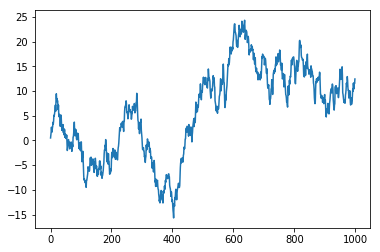
\includegraphics[width=\textwidth]{random_walk_1D.png}
    \caption{1D Time series representation of a Random walk}
    \label{fig:randwalk}
\end{figure}
A random walk is a particular case of an autoregressive moving average time series (ARMA) which are widely used models of time series data.
\subsection{ARMA}
\begin{Def}\label{ARMA}
Let $x_t$ be a time series, it is an autoregressive moving average (ARMA) of order $p$ and $q$ if it satisfies the following : 
\begin{equation*}\label{ARMA(p,q)}
x_{t}=\sum_{i=1}^{p}\phi_ix_{t-i}+\sum_{j=1}^{q}\psi_j\epsilon_{t-j} 
\end{equation*}
where $\phi_i$ and $\psi_j$ are real non zero constants $\forall i,j$ and $\epsilon_t\sim N(0,\sigma)$ are i.i.d
\end{Def}
\begin{ex} Let $\phi_1=0.75$, $\phi_2=-0.25$, $\psi_1=0.65$; $\psi_2=0.35$ define an $ARMA(2,2)$ process. A sample of this process is plotted \ref{fig:ARMA(2,2)_sample}. 
\begin{figure}
    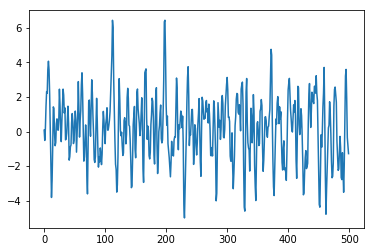
\includegraphics[width=\textwidth]{ARMA(2,2).png}
    \caption{A sample of an ARMA(2,2) process}
    \label{fig:ARMA(2,2)_sample}
\end{figure}
\end{ex}
\begin{Def}\label{backshift}
Let $x_t$ be a time series. The backshift operator $L$ satisfies $Lx_t:=x_{t-1}$
\end{Def}
ARMA processes are composed by two terms, an autoregressive term and a movering average term. 
\begin{Def}Let $L$ be a backshift operator. Let $\phi_i$ be real numbers. The Autoregressive operator $\phi$ satisfies : 
\begin{equation*}
    \phi(L)=1-\sum_{i=1}^{p}\phi_i L^{i}
\end{equation*}
\end{Def}
\begin{Def}
Let $L$ be a backshift operator. Let $\psi_i$ be real numbers and $\psi_0=1$. The Autoregressive operator $\psi$ satisfies : 
\begin{equation*}
    \psi(L)=\sum_{i=0}^{q}\psi_i L^{i}
\end{equation*}
\end{Def}
Thanks to these definitions, one can represent an $ARMA(p,q)$ process in a more compact form : 
\begin{equation*}
    \phi(L)x_t=\psi(L)\epsilon_t
\end{equation*}
\subsection{Invertibility, stability and stationarity}
It appears under this more compact representation that if $\phi$ is invertible (resp. $\psi$) one can go from an ARMA representation to an infinite autoregressive representation (resp. moving average) of the process $x_t$. This is true if the roots of $\phi$ (resp $\psi$) lie outside the unit circle. This can be understood in light of the fundamental theorem of algebra. Indeed, let $\lambda_i$ be the roots of $\phi$ (they are all non zeros by definition of $\phi$). Then \begin{equation*}
    \phi(z)\propto \prod_{i=1}^{p}(1-z/\lambda_i)
\end{equation*}
It appears that $phi$ is invertible if and only if eah factor is invertible, which is equivalent to $|z/\lambda_i|<1$ so the $\lambda_i$ lie outside the unit circle. \newline 
If $\phi$ is invertible the ARIMA process is said to be stable. If $\psi$ is invertible the ARIMA process is said to be invertible.
\begin{Def}
The (cross) autocovariance of a time series $x_t$ is defined by \begin{equation*}
    \gamma_{t,k}=\mathds{E}(X_tX^{t}_{t-k})
\end{equation*}
The (cross) autocorrelation $\Gamma_k$ is : 
\begin{equation*}
    \Gamma_{t,k}=\frac{\gamma_{t,k}}{\gamma_0}
\end{equation*}
\end{Def}
The notion of weak stationarity is a very important one for time series as stable autoregressive processes are stationary : 
\begin{Def} A time series $x_t$ is (weakly) stationary if
\begin{enumerate}
    \item $\mathds{E}(X_t)$ does not depend on time
    \item The autocovariance depends only on the lag $k$
\begin{equation*}
    \gamma_{t,k}=\gamma_k\quad\forall t
\end{equation*}
\end{enumerate}
\end{Def}
It is possible to write an autoregressive model of order $p$  ($AR(p)$) process $x_t$ as an $AR(1)$ by the following trick. Let $U_t=\begin{pmatrix} x_t\\
\cdot\\
\cdot\\
x_{t-p+1}
\end{pmatrix}$ and $W_t=\begin{pmatrix} \epsilon_t\\
\cdot\\
\cdot\\
0
\end{pmatrix}$ Then one derives \begin{equation}\label{VAR_ptoVAR_1}
    U_t=AU_{t-1}+W_t
\end{equation} where $A$ is a squared $p$ real matrix such that : \begin{equation*}
A=\begin{pmatrix} 
\phi_1 & \phi_2 & \cdot & \cdot & \phi_p \\
1  & 0 & \cdot & \cdot & 0\\
0 & 1 & \cdot & \cdot & 0 \\
\cdot & \cdot & \cdot & \cdot \\
\cdot & \cdot & \cdot & \cdot \\
0 & 0 & \cdot & \cdot & 1 \\
0 & 0 &  \cdot & \cdot & 0
\end{pmatrix}
\end{equation*}
\begin{Prop}
Let $\rho(A)$ be t he spectral radius of $A$ i.e. the greatest eigenvalue of $A$. If the spectral Radius $\rho(A)$ of $A$ is less than one then the process is stable.
\end{Prop}
One can easily show this proposition by observing that the characteristic polynomial of $A$ defined by $\det(\lambda -A)$ is proportional to $\det(zA-1)$ for $z=\lambda^{-1}$ which is $\phi$. In other words, if the roots of $\phi$ lie outside the unit circle then all the eigenvalues of $A$ are less than one then $\rho(A)<1$.
\begin{Prop}
A stable $AR(p)$ process is stationary.
\end{Prop}
Indeed if $X_t$ is stable then it writes : 
\begin{equation*}
    X_t=\phi(L)^{-1}\psi(L)\epsilon_t
\end{equation*}
Stability ensures that we can formally expand $X_t$ as an infinite series : 
\begin{equation*}
    X_t=\sum_{i=0}^{\infty}\xi_i\epsilon_{t-i}
\end{equation*}
A direct computation showsthat 
\begin{equation}\label{ACF_MA}
    \gamma_{t,k}=\sum_{i=0}^{\infty}\xi_{i+k}\xi_{i}\sigma^{2}
\end{equation}
Which does not depend on t hence the stationarity of the process. 
\begin{ex}
For example, the following AR($1$) with $\phi_1=0.5$ process is stable :  \begin{equation*}
    x_t=0.5x_{t-1}+\epsilon_t
\end{equation*}
For some natural number $N$, one can write it also as :
\begin{equation*}
    x_t=\phi^N\epsilon_{t-N}+\sum_{i=0}^N\phi^i\epsilon_{t-i}
\end{equation*}
So for N sufficiently large and $\phi$ (spectral radius) strictly less than one the process will converge (exponentially) toward a finite moving average process (stable)\ref{fig:AR(1)_stable_sample}. Conversely if the spectral radius is greater than one, the process will explode (unstable)\ref{fig:AR(1)_unstable_sample}.
\end{ex}
\begin{figure}
    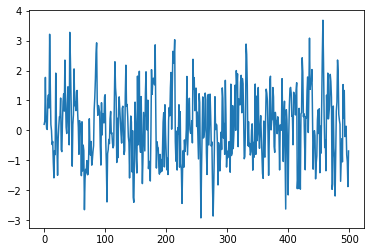
\includegraphics[width=\textwidth]{AR(1)_stable.png}
    \caption{A sample of a stable AR(1) process}
    \label{fig:AR(1)_stable_sample}
\end{figure}
\begin{figure}
    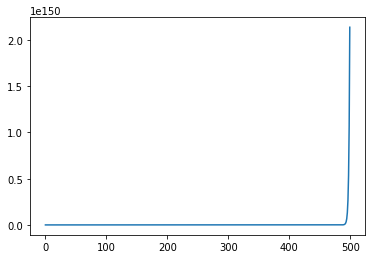
\includegraphics[width=\textwidth]{AR(1)_unstable.png}
    \caption{A sample of an unstable AR(1) process}
    \label{fig:AR(1)_unstable_sample}
\end{figure}
Back to our random walk at the beginning, we see that a random walk is non stationary since the 0-lagged aucorrelation of $X_t$ is exactly $t$ thus it is unstable.
From \ref{ACF_MA} it appears that the autocorrelation function alone gives us enough information about the model order of a finite moving average. However this is not the case if the process has an autoregressive component as for an $AR(1)$ process as the autocovariance satisfies the following recurrent relation : 
\begin{equation*}
    \forall k\in\mathds{N},\quad\gamma_k=\sum_{i=1}^{k-1}\phi_1^i\gamma_{k-i}
\end{equation*}
\begin{Def}
Let $X_{t+1:t+h-1}$ be the  collection of random variables $X_{t+1},X_{t+2},\cdot\cdot,X_{t+h-1}$  Define the partial autocorrelation function as :
\begin{equation*}
    \rho_{h|h-1}=\cor(X_{t+h},X_t|X_{t+1:t+h-1})
\end{equation*}
\end{Def}
\begin{ex}
Let $x_t$ be an $AR(1)$ time series. One derives \begin{align*}
    \mathbb{E}(X_{t+2}|X_{t+1})=\phi X_{t+1}\\
    \mathbb{E}(X_{t}|X_{t+1})=X_{t+1}
\end{align*}
Injecting in the definition of the partial, autocorrelation, \begin{equation*}
\rho_{2|1}=\frac{\mathbb{E}(X_{t+2}-\phi X_{t+1})(X_{t}-X_{t+1})}{\gamma_0}
\end{equation*}
With $\gamma_1=\phi\gamma_0$ and replacing in the previous equation one derives \begin{equation*}
    \rho_{2|1}=\phi
\end{equation*}
We plot an example of the (autocorrelation function) acf and partial autocorrelation function (pacf) of an AR(1) model with $\phi=0.5$ on figure \ref{fig:acf_pacf_AR1}
\begin{figure}[h]
    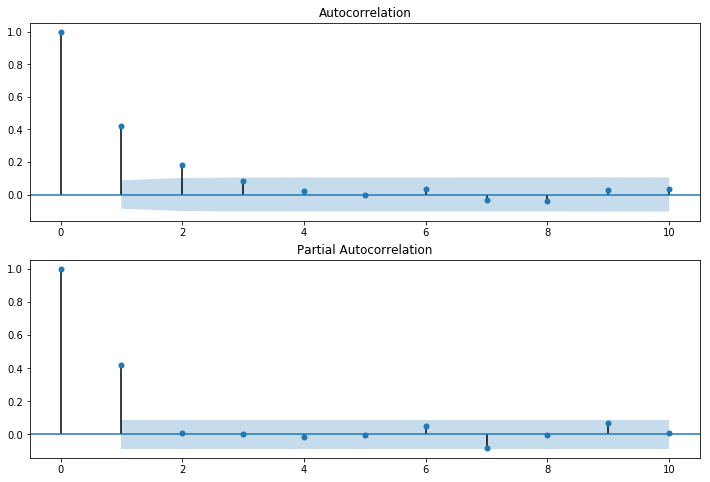
\includegraphics[width=\textwidth]{acf_pacf_AR1.png}
    \caption{ACF and PACF of $AR(1)$, $\phi=0.5$}
    \label{fig:acf_pacf_AR1}
\end{figure}
\end{ex}
The ACF decrease exponentially due to the fact that $\gamma_k=\phi^k\gamma_0$ and the PACF gives indeed a good estimation of the model order. In our case it give exactly the coefficient of the model but it is not a general feature of the pacf as we will see some methods of estimation.
\section{Estimation}
\section{Spectral analysis}
\section{G-causality}
\section{One Example}
\section{Notations}
\section{Questions}
\begin{itemize}
\item Sationarity equivalent to stability equivalent to coefficint does not depend on time?
\end{itemize}
\section{appendix, proofs}
\end{document}
